\documentclass[11pt,letterpaper]{article}
\usepackage[T1]{fontenc}
\usepackage{lmodern}
\usepackage[margin=1in]{geometry}
\usepackage{amsmath,amssymb,amsthm}
\usepackage{booktabs,array}
\usepackage{microtype}
\usepackage{xurl}
\usepackage{tikz}
\usetikzlibrary{positioning,arrows.meta}
\usepackage[colorlinks=true,linkcolor=blue,urlcolor=blue,citecolor=blue]{hyperref}
\newtheorem{theorem}{Theorem}[section]
\newtheorem{lemma}[theorem]{Lemma}
\newtheorem{proposition}[theorem]{Proposition}
\newtheorem{remark}[theorem]{Remark}
\newcommand{\PA}{\mathrm{PA}}
\newcommand{\NN}{\mathbb{N}}
\newcommand{\Con}{\operatorname{Con}}
\newcommand{\Prf}{\operatorname{Prf}}
\newcommand{\Prov}{\operatorname{Prov}}
\newcommand{\code}[1]{\ulcorner #1\urcorner}
\newcommand{\src}[2]{\href{https://github.com/jamesyc/BusyBeaver/blob/main/#1}{\texttt{\nolinkurl{#2}}}}
\newcommand{\repo}[1]{\texttt{\nolinkurl{#1}}}
\setlength{\emergencystretch}{2em}
\title{Two-sided independence from Peano arithmetic\\for a 211-state Turing machine}
\author{}
\date{}
% Omit the author and date blocks, including their vertical space.
\makeatletter
\renewcommand{\@maketitle}{%
  \newpage\null\vskip 2em
  \begin{center}
    {\LARGE \@title\par}
  \end{center}
  \vskip 1em}
\makeatother

\begin{document}
\maketitle
\begin{abstract}
PA211 is a binary Turing machine with 211 working states. It searches for
a contradiction in ordinary first-order Peano arithmetic. This article
describes the machine, relates its execution to PA proofs, and proves
both unprovability claims for its arithmetic nonhalting sentence $N$:
\[
\PA\nvdash N \qquad\text{and}\qquad \PA\nvdash\neg N.
\]
The first conclusion follows from consistency of PA and the checked internal
implication $\PA\vdash N\to\Con(\PA)$. The second uses soundness of PA in
the standard natural numbers, a theorem of ordinary classical mathematics.
The machine-specific proof and the independence corollaries are checked
in Lean~4 on top of Foundation. Their axiom audit reports only
\texttt{propext}, \texttt{Classical.choice}, and \texttt{Quot.sound}.
\end{abstract}

\section*{Outline}

Section~\ref{sec:machine} describes the machine and the program it runs.
Section~\ref{sec:encoding} writes down the arithmetic sentence $N$.
Section~\ref{sec:bridge} connects machine runs to PA proofs in both
directions. Sections~\ref{sec:first-side} and~\ref{sec:two-sided} prove
the two halves of independence. Section~\ref{sec:zero-one} explains why
searching for a proof of $0=1$ is the design already used.
Section~\ref{sec:checked} lists the Lean results.
Figure~\ref{fig:pipeline} shows how a refutation leads to a halting trace.

\begin{figure}[ht]
\centering
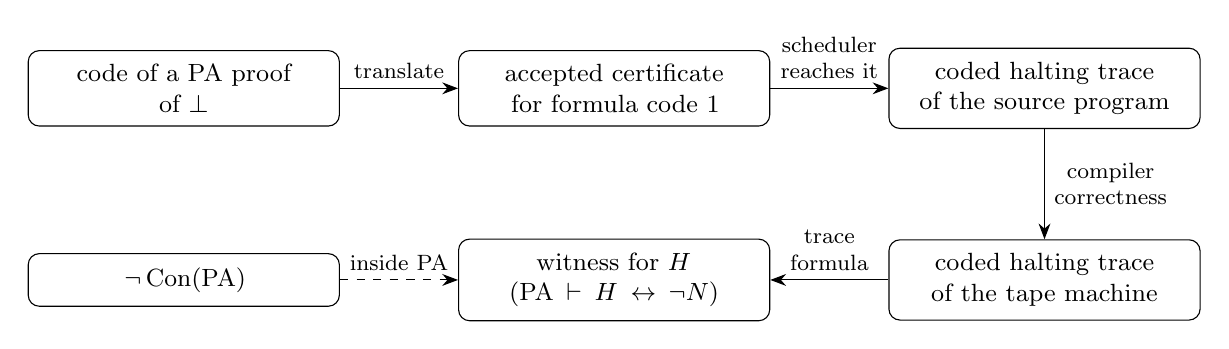
\begin{tikzpicture}[
  box/.style={draw,rounded corners,align=center,inner sep=5pt,font=\small,text width=3.6cm},
  lab/.style={font=\footnotesize,align=center},
  >={Stealth[length=2mm]}]
\node[box] (pa) {code of a PA proof\\of $\bot$};
\node[box,right=1.5cm of pa] (nat) {accepted certificate\\for formula code $1$};
\node[box,right=1.5cm of nat] (src) {coded halting trace\\of the source program};
\node[box,below=1.4cm of src] (tm) {coded halting trace\\of the tape machine};
\node[box,left=1.5cm of tm] (trace) {witness for $H$\\($\PA\vdash H\leftrightarrow\neg N$)};
\node[box,left=1.5cm of trace] (con) {$\neg\Con(\PA)$};
\draw[->] (pa) -- node[lab,above]{translate} (nat);
\draw[->] (nat) -- node[lab,above]{scheduler\\reaches it} (src);
\draw[->] (src) -- node[lab,right]{compiler\\correctness} (tm);
\draw[->] (tm) -- node[lab,above]{trace\\formula} (trace);
\draw[->,dashed] (con) -- node[lab,above]{inside PA} (trace);
\end{tikzpicture}
\caption{The proof of $\PA\vdash N\to\Con(\PA)$. Each arrow is a checked
Lean construction on codes, uniformly in every model of PA; the dashed
arrow summarizes the composite inside PA. In a nonstandard model these
codes can have nonstandard lengths and need not describe actual finite
proofs or runs. In $\NN$, they describe genuine finite objects. The
converse, that consistency gives actual nonhalting, is a separate argument:
soundness of the object calculus, the stack invariant, and positive
progress of the simulation (Section~\ref{sec:bridge}).}
\label{fig:pipeline}
\end{figure}

\section{Main theorem and preliminaries}

Busy Beaver values are defined by Rad\'o~\cite{rado}. Yedidia and
Aaronson~\cite{yedidia} constructed a 7,910-state machine whose
nonhalting is unprovable in ZFC if ZFC is consistent; their argument for
its actual nonhalting uses stronger set-theoretic assumptions. They also
asked how small such machines can be. PA211 addresses this question for
Peano arithmetic. Its proof is
formalized in Lean~4 on top of the Foundation library~\cite{foundation};
the source is~\cite{project}. We make no claim that 211 states is minimal.

Let $\PA$ be ordinary first-order Peano arithmetic with full induction.
The formalization uses Foundation's theory \texttt{Peano}, in the language
of zero, one, addition, multiplication, equality, and order.
Write $\PA\vdash A$ when a finite formal PA proof of $A$ exists, and
$\NN\models A$ when the sentence is true in the standard natural numbers.
Truth alone does not imply provability.

Let $M$ be the exact machine specified in Section~\ref{sec:machine}, and
let $H$ be the repository's arithmetic sentence asserting that $M$ has a
finite halting trace from the blank tape. Define $N:=\neg H$.
In particular, $\neg N$ is classically equivalent to $H$.

\begin{theorem}[Independence of the nonhalting sentence]\label{thm:main}
The machine $M$ does not halt from the blank tape, $\NN\models N$, and
\[
\PA\nvdash N\quad\text{and}\quad\PA\nvdash\neg N.
\]
\end{theorem}

We work in ordinary classical mathematics, where
$\NN\models\PA$ and hence PA is consistent (Lemma~\ref{lem:sound}).
This is not a PA proof of its own consistency or soundness. The two
directions use different hypotheses:
\begin{itemize}
\item \emph{Consistency of PA} gives nonhalting, $\NN\models N$, and
$\PA\nvdash N$ (Proposition~\ref{prop:first}).
\item \emph{Soundness of PA in $\NN$} gives $\PA\nvdash\neg N$
(Proposition~\ref{prop:second}).
\end{itemize}
The Lean endpoint assumes consistency. The two-sided module discharges
both hypotheses with Foundation's proof that $\NN$ models PA.

\section{Definition of PA211}\label{sec:machine}

The tape is infinite in both directions, has alphabet $\{0,1\}$, and is
initially all zero. In the published table the head starts at the origin
in state $0$. The working-state set is
\[
Q=\{0,1,\ldots,214\}\setminus\{122,150,205,214\},\qquad |Q|=211.
\]
State $215$ is the halt label and is not a working state. Each pair in
$Q\times\{0,1\}$ has one transition, giving exactly $422$ rows. A row
$(q,b,b',D,q')$ means: read $b$ in state $q$, write $b'$, move one cell in
direction $D$, and enter $q'$. For example, the first row is
\[
(0,0,1,R,1).
\]
The full table defines $M$:
\src{Lean/data/pa211.tm}{Lean/data/pa211.tm}.
Its SHA-256 digest is
\begin{quote}\small
\nolinkurl{fd986dc8cb7f30c3d9f6e4a1767e3335f06679aeadeedb8d1d7fecd442f232c3}.
\end{quote}
The physical simulation proof uses equivalent sparse labels, with
start label $74$ and halt label $254$. The arithmetic sentence uses the
published labels and exactly the 422 active transitions. Relabeling does
not add states or change halting behavior.

\subsection{Refutation search}

The machine runs a register program that enumerates finite lists of proof
commands in a small first-order calculus. It executes the commands in
order and halts when they derive a fixed false formula. That calculus
proves a contradiction if and only if PA does. The direction from PA
refutations to calculus refutations is arithmetized inside PA. The other
direction is an external theorem, which suffices for this proof. The
following sections describe the calculus, the command interpreter, the
enumeration, and the compilation to a tape machine.

\subsection{The numeric proof calculus}

Formulas are coded by natural numbers using the Cantor pairing
$\langle a,b\rangle=\binom{a+b+1}{2}+b$. Variables are number labels.
If $A,B$ are the formulas decoded from $a,b$, the decoder uses
\[
\begin{aligned}
0 &\mapsto \top,\\
4\langle a,b\rangle &\mapsto A\to B &&(a+b>0,\ b\ne1),\\
4\langle a,1\rangle &\mapsto \neg A,\\
4\langle a,b\rangle+1 &\mapsto x_b\in x_a,\\
4\langle a,b\rangle+2 &\mapsto \forall x_a\,B,\\
4\langle a,b\rangle+3 &\mapsto x_a=x_b.
\end{aligned}
\]
In particular, code $1$ decodes to $x_0\in x_0$, not to a primitive
logical falsity symbol. The numeric constructor for negation is
\texttt{wn a = wim a 1}, and the decoder treats that code specially as
logical negation. These interpretations agree in the intended arithmetic
models because self-membership is false there. The encoding is not
injective on named formulas
(\src{Lean/metamathematics/PA215PA/NativeDecode.lean}{NativeDecode.lean}).
The only nonlogical relation symbols are $\in$ and $=$.

The rules are modus ponens and generalization. The axioms are nine
schemas (\src{Lean/PA215/Source/ActualAXCode.lean}{ActualAXCode.lean}):
quantifier distribution and exchange, instantiation, existence of a
witness for $x_a=x_b$, congruence of $=$ with $\in$, transitivity of $=$,
the single implicational axiom
$((p\to q)\to r)\to((r\to p)\to(s\to p))$ of {\L}ukasiewicz (with the
numeric restriction $u\le a$ in \texttt{rho8 a b c u}), and a guarded
\emph{pointed separation} axiom: for a
set $x_a$, a point $x_b$, and a formula $\varphi$, some $x_c$ contains the
members of $x_a$ satisfying $\varphi$, only elements satisfying $\varphi$,
and $x_b$ if $\varphi(x_b)$.

To prove source soundness, the formalization first derives the literal AX
formulas in the supporting \texttt{NativeCalculus}. The two presentations
are not definitionally identical; their connection is proved in
\src{Lean/metamathematics/PA215PA/ActualAXBridge.lean}{ActualAXBridge.lean}.
The two directions connecting the object calculus to PA use different proofs:
\begin{itemize}
\item \emph{Soundness.} Interpret $y\in x$ as ``bit $y$ of $x$ is $1$''
(Ackermann's coding of hereditarily finite sets) inside any model of PA.
Every derivable formula is true under this interpretation. The formula
$x_0\in x_0$ is false because $y\in x$ implies $y<x$. By completeness,
an actual finite derivation of code $1$ gives $\PA\vdash\bot$. This is an
external theorem about finite derivations, not an internal translation of
proof codes
(\src{Lean/metamathematics/PA215PA/NativeSoundness.lean}{NativeSoundness.lean},
\repo{native_refutation_PA_bottom}).
\item \emph{Completeness for refutations, inside PA.} Numbers are interpreted as
finite von Neumann--style ordinals ($0=\emptyset$, $S a=a\cup\{a\}$), with
equality read as order isomorphism and induction as ordinal induction
using separation. A PA proof of $\bot$ is first translated into an equivalent
presentation of PA with successor, then into a certificate accepted by
the calculus. The translation works on proof codes in every model of PA,
including nonstandard codes
(\src{Lean/metamathematics/PA215PA/FoundationNativeRefutationTransport.lean}{FoundationNativeRefutationTransport.lean}).
\end{itemize}
Deriving code $1$ is therefore the contradiction the machine looks for.

\subsection{Command semantics}

The interpreter state consists of four numbers $(t,w,d,h)$. The registers
$t$ and $h$ hold formula codes, $w$ encodes a stack by iterated pairing,
and $d$ is a label offset. There are three commands
(\src{Lean/metamathematics/PA215PA/CommandSemantics.lean}{CommandSemantics.lean},
\src{Lean/metamathematics/PA215PA/ActualCommandSemantics.lean}{ActualCommandSemantics.lean}):
\begin{center}\small
\begin{tabular}{@{}lp{0.72\linewidth}@{}}
\toprule
Command & Effect \\
\midrule
$\mathsf{shift}$ & If $t+h=1$, halt. Otherwise $t\gets h$ and pop the
top of $w$ into $h$. \\
$\mathsf{mp}\ x$ & Put $y=d+x$. If $h$ codes $t\to y$, then $t\gets y$
(modus ponens) and push $0$; otherwise $t\gets 0$. In both cases
$d\gets y$ and $h\gets 0$. \\
$\mathsf{ax}\ c\ x\ y$ & With parameters $a=d+x$ and $b=h+y$, push eight
axiom instances and the generalization $\forall x_d\,\varphi_h$ of the
formula coded by the incoming $h$, together
with the old $t$; set $t$ to the separation instance (or to truth if $c$
collides with $a$ or $b$) and $d,h\gets0$. \\
\bottomrule
\end{tabular}
\end{center}
The checked invariant \texttt{Invariant} combines \texttt{TopSound}, which
says that $t$ and $h$ are derivable, with \texttt{WrapperStack.Safe}, which
says the same for every stack entry above a fixed initial tail. A $\mathsf{shift}$
halts only if $t+h=1$, so one of the two derivable registers equals $1$,
and code $1$ is derivable (\repo{shift_halt_refutation}). This is the
only halting instruction in the program.

\subsection{Enumeration of command sequences}

A number $n$ decodes to a command list $\mathrm{word}(n)$ by repeated
unpairing
(\src{Lean/PA215/Source/Enumeration.lean}{Enumeration.lean}). The program
executes $\mathrm{word}(0),\mathrm{word}(1),\mathrm{word}(2),\ldots$ in
order, keeping the interpreter state between words. Completeness of the
search follows from two checked facts:
\begin{itemize}
\item every finite command list is a prefix of some $\mathrm{word}(n)$;
\item there is a fixed ``halt word'' (reset, then the compiled
refutation, then $\mathsf{shift}$) that halts from \emph{every} state when
a refutation exists.
\end{itemize}
The stack also retains enough derivable entries to continue:
$\mathsf{ax}$ pushes ten entries and $\mathsf{shift}$ pops one. A counting
argument gives every prefix of the schedule a net weight of at least $-3$
against an initial depth of $9$. If the calculus is consistent, every
command can execute and the program never halts.

\subsection{Simulation by a binary Turing machine}

The enumeration and interpreter are written as a register program with
nine unbounded registers and 3,947 instruction sites. The 211-state
construction rearranges 366 source paths in a 173-node tree. The
ordinal instructions and successors are unchanged, as checked by
\src{Lean/User211SourceEquivalence.lean}{User211SourceEquivalence.lean}. The instructions are
increment, decrement-or-branch-on-zero, structured break and continue,
and a single halt; control returns to the first site after the last
(\src{Lean/PA215/Source/Syntax.lean}{Syntax.lean}).

On the tape, a configuration of the register program is a \emph{frame}:
a marker, the binary path of the current site, padding, and the register
file with each value $v$ written in unary as $0\,1^{v+1}$
(\src{Lean/PA215/Source/RootFrame.lean}{RootFrame.lean}). A \emph{runtime
contract} states that from the frame of a site, the tape machine reaches
the frame of the correct successor site in a positive number of steps.
There is one contract per site and a second one for each of the 1,187
decrement sites, giving $3{,}947+1{,}187=5{,}134$ contracts, each checked
by a certified symbolic executor. Starting from the blank tape, the
machine runs exactly 64,764 steps to a frame of the register program. That
frame is the state the program reaches 159 steps after a fixed seed state,
the entry of the initial command $\mathsf{ax}\ 0\ 0\ 0$.

\begin{remark}
Required support modules retain their original namespaces, including
\texttt{PA213}, \texttt{PA215}, \texttt{PA213PA}, and \texttt{PA215PA}.
They supply the proof calculus, scheduler, and compiler lemmas for PA211.
\end{remark}

\section{Arithmetization of halting}\label{sec:encoding}

A configuration is represented by a state $q$ and two natural numbers
$l,r$. The low binary digit of $r$ is the scanned cell; subsequent digits
describe the tape to its right. The low digit of $l$ is the cell immediately
to the left of the head. Unrepresented high digits are zero. This encodes
every configuration reached in finitely many steps from a blank tape.

For a transition reading $b$ and writing $w$, a right move has the relation
\[
q=q_0\ \land\ q'=q_1\ \land\
\exists t\,(r=2t+b\ \land\ l'=2l+w\ \land\ r'=t).
\]
A left move has the relation
\begin{align*}
q=q_0\ \land\ q'=q_1\ \land\ \exists t,u,e\,(& (e=0\lor e=1)
\land l=2u+e\land r=2t+b\\
&\land l'=u\land r'=2(2t+w)+e).
\end{align*}
Let $F(q,l,r,q',l',r')$ be the disjunction of these relations over the
422 rows. The relations are defined in
\src{Lean/metamathematics/User211PAStepFormula.lean}{User211PAStepFormula.lean},
restricted to the active rows by
\src{Lean/metamathematics/User211EndpointExactHaltingFormula.lean}{User211EndpointExactHaltingFormula.lean}.

Using the repository's arithmetic relation for sequence access, write
$(q_i,l_i,r_i)$ for the $i$th entries of three coded sequences. Then $H$
is the following formula, with sequence notation expanded into arithmetic:
\begin{equation}\label{eq:trace}
\exists n,\vec q,\vec l,\vec r\;
\left[
\begin{aligned}
&q_0=0\land l_0=0\land r_0=0\land q_n=215\ \\
&{}\land\forall i<n\;F(q_i,l_i,r_i,q_{i+1},l_{i+1},r_{i+1})
\end{aligned}\right].
\end{equation}
The arrows denote number codes, not second-order sequence variables.
The Lean definition explicitly quantifies the entries and relates them to
the codes using \texttt{nthDef}. Equation~\eqref{eq:trace} abbreviates that
definition of the exact sentence used in the proof.

The checked arithmetic adequacy theorem and the literal-to-sparse run
conjugacy establish
\begin{equation}\label{eq:adequacy}
\NN\models N\quad\Longleftrightarrow\quad
M\text{ does not halt from its blank initial configuration}.
\end{equation}
An auxiliary encoding has four padding states and 430 rows. An invariant
valid in every PA model proves those states unreachable, giving the
required equivalence with the exact 422-row sentence.

\section{Correctness of the refutation search}\label{sec:bridge}

The external simulation proves nonhalting. A separate implication inside
PA lets us apply the second incompleteness theorem.

\subsection{Nonhalting from consistency}

The source program has 3,947 instruction sites. A checked startup of
64,764 tape steps reaches a frame corresponding to a 159-step prefix of
that source. The compilation proof uses 5,134 runtime contract records.
At each reachable instruction frame it proves that a positive, finite
number of tape steps implements the next source instruction.

If PA is consistent, soundness of the object calculus rules out a
derivation of code $1$, so the search continues. The simulation takes at
least one tape step per source instruction: after $k$ instructions, at
least $k$ tape steps have occurred. If the machine halted after $t$ tape steps, simulation of
another sufficiently long finite source prefix would give a run longer
than $t$ from the same deterministic initial configuration, a
contradiction. The checked theorem is
\begin{equation}\label{eq:external}
\Con(\PA)\quad\Longrightarrow\quad M\text{ does not halt}.
\end{equation}
Here $\Con(\PA)$ is read externally as absence of an actual PA refutation.
The source-to-machine theorem is \repo{consistent_literal_nonhalting} in
\src{Lean/metamathematics/User211ConsistentNonhalting.lean}{User211ConsistentNonhalting.lean}.
Together with~\eqref{eq:adequacy}, it gives $\NN\models N$ under consistency.

\subsection{Internal consistency implication}

Choose the standard arithmetized PA proof predicate, and put
\[
\Prov_{\PA}(x):=\exists p\,\Prf_{\PA}(p,x),\qquad
\Con(\PA):=\neg\Prov_{\PA}(\code{\bot}).
\]
The following argument is formalized in every model of PA.
A code for a PA refutation is translated into a refutation code accepted
by the actual numeric checker. The scheduler reaches that code, and its
source execution is converted to a tape trace. Adding the startup prefix
gives a trace from the blank initial configuration. In particular,
\[
\PA\vdash \Prov_{\PA}(\code{\bot})\to H,
\qquad\text{hence}\qquad
\boxed{\PA\vdash N\to\Con(\PA).}
\]
The proof first uses the auxiliary trace, then eliminates its padding
states. First-order completeness gives a PA derivation because the
implication holds in all PA models, including nonstandard ones.
Equivalence in the standard model alone would not suffice.

The relevant source files are
\src{Lean/metamathematics/PA215PA/FoundationNativeRefutationTransport.lean}{FoundationNativeRefutationTransport.lean},
\src{Lean/metamathematics/User211RefutationHalting.lean}{User211RefutationHalting.lean},
and \src{Lean/metamathematics/User211NonhaltingUnprovability.lean}{User211NonhaltingUnprovability.lean}.
The argument uses only the displayed internal implication.

\section{Unprovability of nonhalting}\label{sec:first-side}

\begin{proposition}\label{prop:first}
If PA is consistent, then $\PA\nvdash N$.
\end{proposition}
\begin{proof}
If $\PA\vdash N$, the internal implication of
Section~\ref{sec:bridge} gives $\PA\vdash\Con(\PA)$ by modus ponens.
G\"odel's second incompleteness theorem~\cite{goedel} for the standard PA
provability predicate forbids this when PA is consistent. In Lean, the
internal implication is stated for the sentence
\repo{PA215.PA.consistencySentence}, and the incompleteness step
(\repo{unprovable_of_internal_consistency_implication}) is applied to
that same sentence, so no identification of two consistency formulas is
needed.
\end{proof}

Abbreviate
$\Prov_{\PA}(\code A)$ by $\Box A$. Standard provability satisfies:
\begin{align*}
\PA\vdash A&\ \Longrightarrow\ \PA\vdash\Box A,\\
\PA&\vdash\Box(A\to B)\to(\Box A\to\Box B),\\
\PA&\vdash\Box A\to\Box\Box A.
\end{align*}
The diagonal lemma supplies $G$ with
$\PA\vdash G\leftrightarrow\neg\Box G$. If PA proved $G$, it would
prove both $\Box G$ and $\neg\Box G$, contrary to consistency.
Internally, the displayed derivability conditions give
\[
\Box G\to\Box\neg\Box G,\qquad
\Box G\to\Box\Box G,\qquad
\Box G\to\Box\bot.
\]
Thus PA proves $\neg\Box\bot\to\neg\Box G$, and hence
$\Con(\PA)\to G$. A PA proof of consistency would therefore give a
PA proof of $G$, which was just ruled out. The project imports the
formal second incompleteness theorem through
\src{Lean/metamathematics/PA215PA/Foundation.lean}{Foundation.lean};
the diagonal lemma and derivability conditions belong to that general
result and require no further facts about PA211.

\section{Unprovability of halting}\label{sec:two-sided}

\begin{lemma}[Soundness of PA in the standard model]\label{lem:sound}
In ordinary classical set theory, for every arithmetic sentence $A$,
\[
\PA\vdash A\quad\Longrightarrow\quad\NN\models A.
\]
In particular, PA is consistent.
\end{lemma}
\begin{proof}
Interpret zero, one, addition, multiplication, and order by their usual
operations and relation on $\NN$. The noninduction axioms of PA hold in
this structure. For any first-order formula $\varphi(x,\vec y)$ and any
assignment of natural numbers $\vec a$ to its parameters, consider its
induction instance. If $\varphi(0,\vec a)$ holds and
$\varphi(n,\vec a)$ implies $\varphi(n+1,\vec a)$ for every $n$, ordinary
induction in the surrounding mathematics gives $\varphi(n,\vec a)$ for
every natural number $n$. Thus every induction axiom is true under every
assignment, so $\NN\models\PA$.

Logical axioms are valid, and the inference rules preserve truth under
all assignments: in particular, modus ponens preserves truth and
generalization preserves validity with the usual variable restrictions.
Induction on the length of a finite derivation therefore proves that
every PA theorem is true in $\NN$. Since $\bot$ is false in $\NN$, it
cannot be a PA theorem.
\end{proof}

The proof takes place in the surrounding set theory, where $\NN$ is a
set-sized structure. PA has not proved its own soundness or consistency,
so the second incompleteness theorem still applies.

\begin{proposition}\label{prop:second}
If PA is sound in $\NN$, then $\PA\nvdash\neg N$; equivalently,
$\PA\nvdash H$.
\end{proposition}
\begin{proof}
Soundness implies consistency. By~\eqref{eq:external} and
\eqref{eq:adequacy}, the machine does not halt and $\NN\models N$.
If $\PA\vdash\neg N$, soundness would give $\NN\models\neg N$,
contradicting $\NN\models N$. Classical double-negation elimination
identifies provability of $\neg N=\neg\neg H$ with provability of $H$.
\end{proof}

\begin{proof}[Proof of Theorem~\ref{thm:main}]
Soundness supplies consistency. The checked nonhalting and adequacy
results give actual nonhalting and truth of $N$.
Proposition~\ref{prop:first} excludes a PA proof of $N$;
Proposition~\ref{prop:second} excludes a PA proof of its negation.
Lemma~\ref{lem:sound} establishes the soundness premise in the stated
metatheory, completing both directions.
\end{proof}

\subsection{Consistency and soundness assumptions}

Consistency alone says that a theory has no derivation of a contradiction.
It does not imply that the theory's existential arithmetic theorems have
standard witnesses. A classical proof of ``there exists
a halting trace'' need not yield a specific standard trace just by
inspecting that proof. We use soundness for the second direction.

For example, if PA is consistent, then
$\PA+\neg\Con(\PA)$ is consistent: otherwise the deduction theorem
would give $\PA\vdash\Con(\PA)$, contradicting the second theorem.
Yet this extension asserts the existence of a PA refutation when there
is no standard such refutation. This extension is consistent but unsound;
the example does not say that PA itself proves $\neg\Con(\PA)$.

For a conventional $\Sigma_1$ halting formula, $\Sigma_1$-soundness is
enough to exclude a proof of false halting. To use that weaker hypothesis
for this exact sentence, one must also establish its PA-provable
equivalence to the chosen $\Sigma_1$ presentation. The proof above uses
full soundness and therefore needs no additional syntactic normalization
claim about \texttt{ExactHaltingFormula.traceSentence}.

Rosser's theorem gives two-sided undecidable sentences from consistency
alone by comparing proofs of a sentence with earlier proofs of its
negation \cite{rosser}. A Rosser-based search would require a different
specification and verified implementation before it could be attributed
to a concrete small machine. No 211-state bound for such a modification
is asserted here.

\section{Choice of refutation target and state complexity}\label{sec:zero-one}

For an ideal exhaustive proof search $M_{\bot}$, the intended equivalence is
\[
M_{\bot}\text{ halts}
\quad\Longleftrightarrow\quad
\exists p\,\Prf_{\PA}(p,\code{0=1})
\quad\Longleftrightarrow\quad \neg\Con(\PA).
\]
Its \emph{nonhalting} therefore expresses consistency. PA proves
$0\ne1$, so a proof of $0=1$ gives a contradiction. Conversely, a
contradiction gives $0=1$ by classical logic. The two finite
proof transformations can be arithmetized in PA.

More generally, replacing falsity by a fixed $B$ has the same property
when $\PA\vdash\neg B$. Merely knowing externally that $B$ is false
does not suffice: a false sentence may itself be undecidable in PA.
For this reduction, ``known false'' must mean ``PA-refutable''.

PA211 already uses this design: it halts when it derives the fixed
refutable formula with code $1$, namely $x_0\in x_0$, and its halting test is
the single comparison $t+h=1$ (Section~\ref{sec:machine}). The target is
already a contradiction, not a sentence such as $\neg\Con(\PA)$. The
object calculus has no arithmetic symbols, so $0=1$ is not one of its
formulas. A PA-refutable target would pass through the same translation.
Changing the target alone does not establish a state reduction: logically
equivalent proof targets can have different compiled state counts. A reduction
would require a concrete revised checker, scheduler, encoding, or
compiler, followed by a new transition table and corresponding proofs.
No such reduction is established here, and 211 states is not claimed to
be minimal.

\section{Formal verification and reproducibility}\label{sec:checked}

The Lean proof checks the source construction, the physical runtime,
the all-model runtime, and the final endpoint. The verification summary
records the package builds and axiom audits \cite{verification}.

The model proof checks the new table and source paths in every PA model
before composing them with the retained scheduler, proof-code translation,
and second incompleteness theorem.

\noindent\begin{minipage}{\linewidth}
The final audit checks the following nine declarations. Names in the
table are relative to \texttt{PA211.UserCandidate.PA}.
\begin{center}\small
\begin{tabular}{@{}p{0.49\linewidth}p{0.45\linewidth}@{}}
\toprule
Theorem & Checked conclusion \\
\midrule
\repo{literal_final_endpoint} & Counts, literal blank nonhalting, truth and unprovability under consistency. \\
\repo{consistent_literal_nonhalting} & Consistency implies nonhalting of the literal table from state 0. \\
\repo{InternalUnprovability.nonhalting_true} & Consistency implies $\NN\models N$. \\
\repo{InternalUnprovability.pa_proves_nonhalting_consistency} & $\PA\vdash N\to\Con(\PA)$. \\
\repo{InternalUnprovability.nonhalting_unprovable} & Consistency implies $\PA\nvdash N$. \\
\repo{literal_arithmetic_binding} & Active arithmetic rows equal the literal transition rows. \\
\repo{Independence.nonhalting_irrefutable} & Consistency implies $\PA\nvdash\neg N$, using soundness. \\
\repo{Independence.two_sided_independence} & $\PA\nvdash N$ and $\PA\nvdash\neg N$, with no explicit premises. \\
\repo{Independence.machine_nonhalting} & Literal blank-tape nonhalting, with no explicit premises. \\
\bottomrule
\end{tabular}
\end{center}
\end{minipage}\par\medskip

The final three declarations are proved in
\repo{Lean/metamathematics/PA211PA/TwoSidedIndependence.lean}, using
Foundation's \texttt{Arithmetic.models\_Peano} and
\texttt{Theory.Proof.sound}. PA consistency and soundness are proved in
Lean's metatheory, not asserted as PA theorems. The audit permits only
\texttt{propext}, \texttt{Classical.choice}, and \texttt{Quot.sound}; the
literal arithmetic binding itself has no axioms.

Run \texttt{bash scripts/check.sh} from the repository root for package
and input checks. After installing the pinned Lean 4.35.0 dependencies
and the two Foundation proof repairs described in
\repo{docs/reproduction.md}, run \texttt{bash scripts/check.sh --full}.
The serial scheduler builds the proof dependencies and independence
corollaries, then audits the nine endpoint declarations. The default
packages are \texttt{PA211} and \texttt{PA211PA}. The core physical
package has a separate eight-root audit.

\begin{thebibliography}{9}
\small
\bibitem{project}
\emph{Nonhalting and PA-independence for a 211-state Turing
machine}. The current publication and its proof dependencies.
\url{https://github.com/jamesyc/BusyBeaver}.

\bibitem{verification}
\emph{PA211 verification}. Package checks, build results, and axiom audits.
\src{docs/validation.md}{docs/validation.md}.

\bibitem{goedel}
Kurt G\"odel. \emph{\"Uber formal unentscheidbare S\"atze der Principia
Mathematica und verwandter Systeme I}. Monatshefte f\"ur Mathematik und
Physik 38 (1931), 173--198.
\url{https://doi.org/10.1007/BF01700692}.

\bibitem{rosser}
J.~Barkley Rosser. \emph{Extensions of some theorems of G\"odel and Church}.
Journal of Symbolic Logic 1 (1936), 87--91.
\url{https://doi.org/10.2307/2269028}.

\bibitem{rado}
Tibor Rad\'o. \emph{On non-computable functions}. Bell System Technical
Journal 41 (1962), 877--884.
\url{https://doi.org/10.1002/j.1538-7305.1962.tb00480.x}.

\bibitem{yedidia}
Adam Yedidia and Scott Aaronson. \emph{A relatively small Turing machine
whose behavior is independent of set theory}. Complex Systems 25 (2016),
297--327. \url{https://arxiv.org/abs/1605.04343}.

\bibitem{foundation}
FormalizedFormalLogic. \emph{Foundation: formalized mathematical logic in
Lean~4}. \url{https://github.com/FormalizedFormalLogic/Foundation}.

\end{thebibliography}
\end{document}
